\chapter{Introdução}

A introdução eu devo escrever por último, deve conter a importancia do projeto, devo descrever o problema e a solução: "existe um problema e foi resolvido assim". O final da introdução deve descrever a estrutura dos capitulos dando uma pincelada rapida em cada um.

\chapter{Conceitos}
\section{Arquitetura de Software}
\section{Atributos de Modularidade}
\subsection{Acoplamento}
\subsection{Coesão}

\chapter{Implementação do Extrator}

Neste capítulo deve documentar o que fiz e como fiz, as dificuldades encontradas no processo, etc...

\section{egypt}

Aqui GCC \sigla{GCC}{GNU C Compiler} ...

O GCC é... \sigla{GCC}.

egypt é um programa originalmente desenvolvido por Andreas Gustafsson\footnote{http://www.gson.org/egypt} para gerar gráfico de chamada entre funções de programas escrito em C, ele funciona lendo os arquivos intermediários gerados pelo GCC e converte isto num gráfico de chamada no formato usado pelo Graphviz\footnote{http://www.graphviz.org}, programa de visualização de gráficos.

O egypt é software livre e em Janeiro de 2009 começou a ser restruturado por Antonio A S. Terceiro o qual tem mantido em\footnote{http://github.com/terceiro/egypt}. As principais mudanças sofridas pelo egypt foram\cite{StructuralComplexityEvolution}:

%\begin{itemize}
%\item Implementation of variables usage detection, to identify which functions use which variables. This is used for calculating both coupling between modules (in the case where modules use variables from other modules) and lack of cohesion for a given module.
%\item Addition of an option to group the calls and variable usages by module, so that we can have a module dependency view. The original egypt only pro- duced graphs at the function level, which makes it impossible to understand the structure of non-trivial software.
%\item Refactoring of the egypt script into an object-oriented design to be able to plug different extraction and reporting modules.
%\item Implementation of a metrics output which, instead of producing Graphviz in-put files, produces a metrics report on the extracted design including coupling and cohesion data.
%\end{itemize}

tool support for extracting coupling and cohesion data from C programs

egypt is program originally developed by Andreas Gustafsson . It works by
reading intermediate files generated by the GCC and producing
as output a call graph in the format used by the Graphviz graph visualization
software 3 , so we can visualize the call dependencies between functions in C
source code.


\section{Doxygen (e a sua API)}


\section{Implementação do Extrator usando a API do Doxygen}

\chapter{Avaliação}
\section{Procedimento}
\section{Resultados}

Nos resultados eu posso comparar o que consegui com a nova ferramenta comparado ao modo antigo do egypt extrair informacoes.

\begin{figure}[h]
\center
\subfigure[ristretto-0.0.1-doxyparse][Egypt::Extrator::Doxyparse]{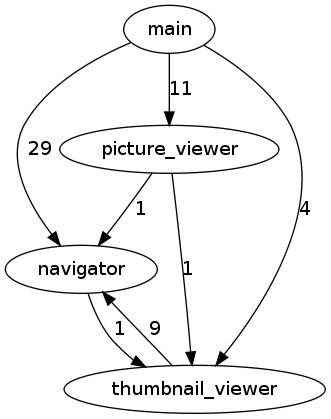
\includegraphics[scale=0.5]{imagens/ristretto-0_0_1-doxyparse}}
\qquad
\subfigure[ristretto-0.0.1-gcc][Egypt::Extrator::GCC]{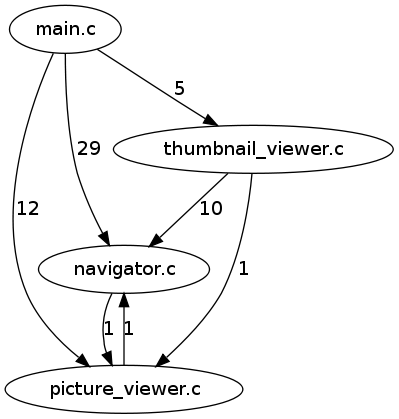
\includegraphics[scale=0.5]{imagens/ristretto-0_0_1-gcc}}
\caption{gráfico de chamada entre módulos do {\bf Ristretto 0.0.1} gerado pelo Egypt}
\end{figure}

\begin{figure}[h]
\center
\subfigure[ristretto-0.0.11-doxyparse][Egypt::Extrator::Doxyparse]{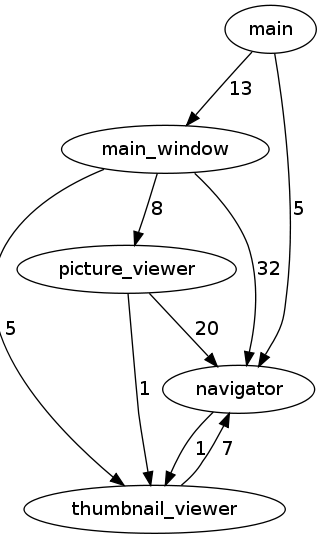
\includegraphics[scale=0.5]{imagens/ristretto-0_0_11-doxyparse}}
\qquad
\subfigure[ristretto-0.0.11-gcc][Egypt::Extrator::GCC]{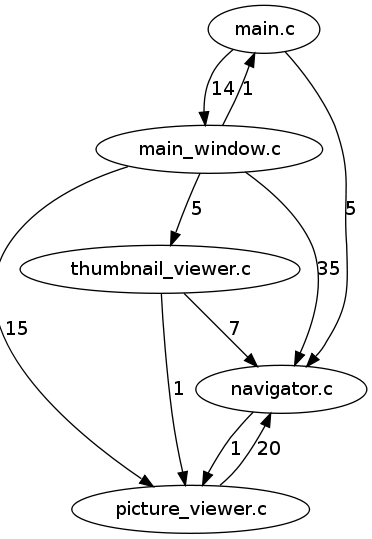
\includegraphics[scale=0.5]{imagens/ristretto-0_0_11-gcc}}
\caption{gráfico de chamada entre módulos do {\bf Ristretto 0.0.11} gerado pelo Egypt}
\end{figure}

\begin{figure}[h]
\center
\subfigure[ristretto-0.0.21-doxyparse][Egypt::Extrator::Doxyparse]{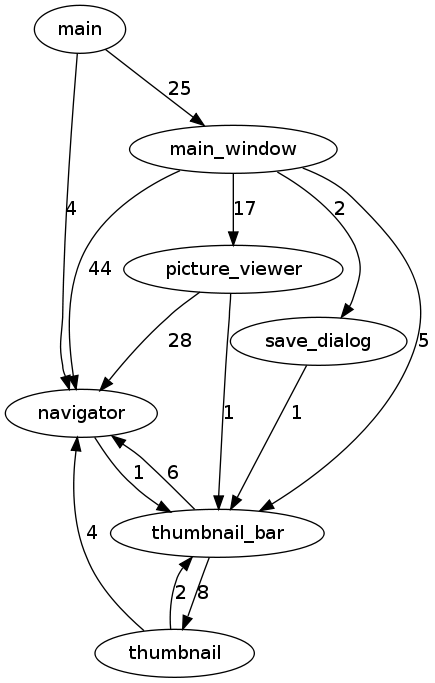
\includegraphics[scale=0.5]{imagens/ristretto-0_0_21-doxyparse}}
\qquad
\subfigure[ristretto-0.0.21-gcc][Egypt::Extrator::GCC]{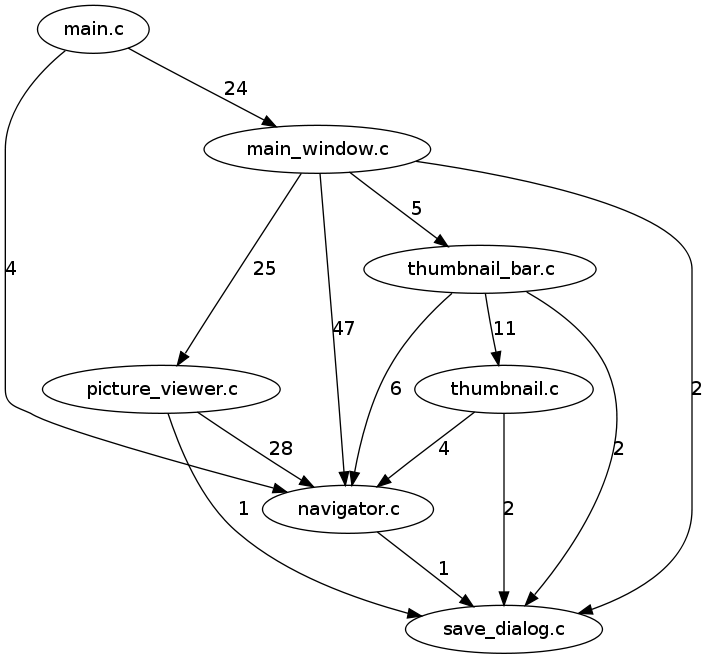
\includegraphics[scale=0.5]{imagens/ristretto-0_0_21-gcc}}
\caption{gráfico de chamada entre módulos do {\bf Ristretto 0.0.21} gerado pelo Egypt}
\end{figure}

\section{Discussão}

\chapter{Conclusão}

A conclusão eu devo escrever por último, deve conter algo assim: "Este trabalho tinha objetivo tal e atingiu tal objetivo". Deve ter referencia de como foi feito e se os resultados foram bons, medios, satisfatorios, ruins, etc. E ao final deve ter trabalhos futuros que eu tenha interesse ou não de fazer.
